% if you need to pass options to natbib, use, e.g.:
%     \PassOptionsToPackage{numbers, compress}{natbib}
% before loading neurips_2019

% ready for submission
% \usepackage{neurips_2019}

% to compile a preprint version, e.g., for submission to arXiv, add add the
% [preprint] option:
%     \usepackage[preprint]{neurips_2019}


% to avoid loading the natbib package, add option nonatbib:
%\usepackage[nonatbib, final]{neurips_2019}

\usepackage[utf8]{inputenc} % allow utf-8 input
%\usepackage[T1]{fontenc}    % use 8-bit T1 fonts
\usepackage{hyperref}       % hyperlinks
\usepackage{url}            % simple URL typesetting
\usepackage{booktabs}       % professional-quality tables
\usepackage{amsfonts,amsmath}       % blackboard math symbols
\usepackage{nicefrac}       % compact symbols for 1/2, etc.
\usepackage{microtype}      % microtypography

%\usepackage[dvipsnames,svgnames]{xcolor}
\usepackage[normalem]{ulem}
\newif{\ifhidecomments}
\usepackage{tumcolors}

\usepackage{tikz,pgf}
\usetikzlibrary{calc}
\usetikzlibrary{fit}
\usetikzlibrary{positioning}

\usepackage{pgfplotstable}

\usepackage{subcaption}

%%%%%%%%%%%%%%%%%%%%%%%%%%%%%%%%%%%%%%%%%%%%%%%%%%%%%%%%%%%%%%%%%%%%%%
%%% Blbliography
%\usepackage[
%  backend=biber,
%  style=authoryear-comp,
%  %  style=numeric,
%  sortcites=true,
%  %   sorting=ydnt,
%  maxnames=3,
%  minnames=1,
%  maxbibnames=99,
%  hyperref=true,
%  %  dashed=false,
%  url=false,
%  isbn=false,
%  doi=false,
%  %  backref=false,
%  uniquename=false,
%]{biblatex}

\usepackage[capitalize, noabbrev]{cleveref}
\usepackage{csquotes}
\usepackage{enumitem}

\usetikzlibrary{fit,positioning}%
\tikzset{%
  % that's a hack ... but I like it´
  node distance/.append code={
    \pgfkeyssetvalue{/tikz/node distance value}{#1}
  },
}%
\tikzset{%
  every node/.append style={
    align=center,
  },
  block/.style={%
    draw,
    rounded corners,
  },%
  input/.style={
  },
  encoder/.style={
    block,
    fill=zombie,
  },
  fc/.style={
    block,
    fill=martini,
  },
  attention/.style={
    block,
    fill=calypso,
    minimum width=3cm,
  },
  mlp/.style={
    block,
    fill=aquaisland,
  },
  operation/.style={
    circle,
    draw,
    text width=3mm,
  },
  add/.style={
    operation, inner sep=2pt,
    node contents={$+$},
%     label={[center]0:$+$},
  },
  mult/.style={
    operation, inner sep=2pt,
    node contents={$\cdot$},
%     label={[center]0:$+$},
  },
  arrow/.style={
    -latex,rounded corners,
  }
}%


\pgfplotsset{select coords between index/.style 2 args={
  x filter/.code={
    \ifnum\coordindex<#1\def\pgfmathresult{}\fi
    \ifnum\coordindex>#2\def\pgfmathresult{}\fi
  }
}}

\pgfplotsset{
  bar/.style={
    draw=none,
  },
  freq bar/.style={
    bar,
    %    fill=tumblue,
  },
  crop bar/.style={
    width=1.1\linewidth,
    width=1.25\linewidth,
    ybar=0.0mm,
    bar width=1.25mm,
    axis x line*=bottom,
    axis y line*=left,
    y axis line style={draw=none},
    ymajorgrids=true,
    enlarge x limits={abs=2mm},
    enlarge y limits=true,
    major grid style={draw=tumivory},
    ytick style={draw=none},
    x tick label style={font=\tiny, rotate=55, anchor=east, inner sep=0pt},
    y tick label style={font=\tiny},
    xlabel near ticks,
    ylabel near ticks,
    xlabel={crop type class},
    ylabel={relative occurrence},
    label style={font=\scriptsize},
    legend style={
      legend columns=-1,
      font=\scriptsize,
      draw=none,
    },
  },
}

\captionsetup{subrefformat=parens}
\captionsetup[table]{skip=10pt}
%%%%%%%%%%%%%%%%%%%%%%%%%%%%%%%%%%%%%%%%%%%%%%%%%%%%%%%%%%%%%%%%%%%%%%
%%% some handy macros

\let\etal\undefined
\makeatletter
\newcommand*{\etal}{%
  \@ifnextchar{.}
  {\textit{et\,al}}
  {\@ifnextchar{,}
    {\textit{et\,al}.}
    {\textit{et\,al}.\,}}%
}
\newcommand{\ia}{\textit{i{.}a{.}}, }
\newcommand{\ie}{\textit{i{.}e{.}}, }
\newcommand{\eg}{\textit{e{.}g{.}}, }
\newcommand{\cf}{\textit{cf{.}}\,}
\newcommand{\vs}{\textit{vs{.}}\,}
\newcommand{\wrt}{wrt.{}\,}
\newcommand{\iid}{iid.}


%%%%%%%%%%%%%%%%%%%%%%%%%%%%%%%%%%%%%%%%%%%%%%%%%%%%%%%%%%%%%%%%%%%%%%%
%%%% Blbliography

\DeclareNameAlias{sortname}{first-last}

\makeatother
\renewcommand*{\nameyeardelim}{\addcomma\addspace}
\DefineBibliographyStrings{english}{%
  andothers = {\etal\isdot}
}

\addbibresource{bib/bib.bib}
%%%%%%%%%%%%%%%%%%%%%%%%%%%%%%%%%%%%%%%%%%%%%%%%%%%%%%%%%%%%%%%%%%%%%%



\usepackage[detect-all, binary-units]{siunitx}
\usepackage{xspace}

%%% text notation

\newcommand{\dictionary}[1]{\texttt{#1}\xspace}
\newcommand{\filename}[1]{\texttt{#1}\xspace}
\newcommand{\tilename}[1]{\texttt{#1}\xspace}

\newcommand{\programminglanguage}[1]{\textsc{#1}\xspace}
\newcommand{\python}{\programminglanguage{Python}}
\newcommand{\pytorch}{\programminglanguage{PyTorch}}
\newcommand{\numpy}{\programminglanguage{NumPy}}
\newcommand{\geojson}{\programminglanguage{GeoJSON}}

\newcommand{\brand}[1]{\textsc{#1}\xspace}
\newcommand{\satellitename}[1]{\brand{#1}}
\newcommand{\sentinel}{\satellitename{Sentinel-2}}
\newcommand{\github}[1]{\brand{GitHub}}

\newcommand{\extref}[1]{\textsl{#1}}

%%% math notation

% operators and functions
\newcommand{\FC}{\ensuremath{\operatorname{FC}}}
\newcommand{\MLP}{\ensuremath{\operatorname{MLP}}}

% symbols
\newcommand{\NObservations}{\ensuremath{T}}
\newcommand{\NBands}{\ensuremath{C}}
\newcommand{\NPixels}{\ensuremath{N}}
\newcommand{\figArchitecture}{%
\begin{figure}[t]
  \centering
  \subcaptionbox{The temporal attention encoder according to the presented paper, where the values $v$ are not calculated specifically, but the sum of $e$ and $p$ is directly passed through to the dot product.\label{fig:tae_transformer_garnot}}{% \usetikzlibrary{fit,positioning}%
\tikzset{%
  % that's a hack ... but I like it´
  node distance/.append code={
    \pgfkeyssetvalue{/tikz/node distance value}{#1}
  },
}%
\tikzset{%
  every node/.append style={
    align=center,
  },
  block/.style={%
    draw,
    rounded corners,
  },%
  input/.style={
  },
  encoder/.style={
    block,
    fill=zombie,
  },
  fc/.style={
    block,
    fill=martini,
  },
  attention/.style={
    block,
    fill=calypso,
    minimum width=3cm,
  },
  mlp/.style={
    block,
    fill=aquaisland,
  },
  operation/.style={
    circle,
    draw,
    text width=3mm,
  },
  add/.style={
    operation, inner sep=2pt,
    node contents={$+$},
%     label={[center]0:$+$},
  },
  mult/.style={
    operation, inner sep=2pt,
    node contents={$\cdot$},
%     label={[center]0:$+$},
  },
  arrow/.style={
    -latex,rounded corners,
  }
}%


\pgfplotsset{select coords between index/.style 2 args={
  x filter/.code={
    \ifnum\coordindex<#1\def\pgfmathresult{}\fi
    \ifnum\coordindex>#2\def\pgfmathresult{}\fi
  }
}}

\pgfplotsset{
  bar/.style={
    draw=none,
  },
  freq bar/.style={
    bar,
    %    fill=tumblue,
  },
  crop bar/.style={
    width=1.1\linewidth,
    width=1.25\linewidth,
    ybar=0.0mm,
    bar width=1.25mm,
    axis x line*=bottom,
    axis y line*=left,
    y axis line style={draw=none},
    ymajorgrids=true,
    enlarge x limits={abs=2mm},
    enlarge y limits=true,
    major grid style={draw=tumivory},
    ytick style={draw=none},
    x tick label style={font=\tiny, rotate=55, anchor=east, inner sep=0pt},
    y tick label style={font=\tiny},
    xlabel near ticks,
    ylabel near ticks,
    xlabel={crop type class},
    ylabel={relative occurrence},
    label style={font=\scriptsize},
    legend style={
      legend columns=-1,
      font=\scriptsize,
      draw=none,
    },
  },
}%
\begin{tikzpicture}[
  node distance=5mm and 1cm,
]
  % creating all nodes

  % the encoder node
  \node[encoder] (encoder) {encoding};

  % the fc nodes
  \node[fc, right=50mm of encoder] (fc1) {$\FC_q$};
  \node[fc, above=of fc1] (fc2) {$\FC_k$};

  \node (add) [add, at=($(encoder.east)!0.35!(fc1.west)$)];
  \node[below=2*\pgfkeysvalueof{/tikz/node distance value} of add] (pos_enc) {positional encoding};
  
  % the attention module was as large as both FC modules ... here's how you can do that
  \path 
    let \p{1}=(fc1.south), 
        \p{2}=(fc2.north), 
        \n{y dist}={abs(\y{2}-\y{1})} 
   in node[attention, right=of fc1.south east, anchor=south west, minimum height=\n{y dist}] (attention) {attention};

  \node (mult) [mult, below=of attention];
  \node[mlp, below=of mult] (mlp) {$\MLP$};

  \node[input, left=of encoder] (input) {input};

  % connecting nodes
  \draw[arrow] (input) -- (encoder);
  \draw[arrow] (encoder) -- node[above] {$e$} (add);
  \draw[arrow] (add) -- node[above, pos=.25] {$(e+p)$} (fc1);
  \draw[arrow] ($(add)!.5!(fc1)$) |- (fc2);

  \draw[arrow] (fc1) --node[above] {$q$} (fc1 -| attention.west);
  \draw[arrow] (fc2) --node[above] {$k$} (fc2 -| attention.west);

  \draw[arrow] (attention) -- node[right] {$a$} (mult);
  \draw[arrow] ($(add)!.5!(fc1)$) |- node[pos=.75, above] {$v=(e+q)$} (mult);

  \draw[arrow] (mult) -- (mlp);
  \draw[arrow] (mlp) -- ++(0,-5mm);

  \draw[arrow] (pos_enc) -- node[right] {$p$} (add);
\end{tikzpicture}
}
  \subcaptionbox{Our adaption of the temporal attention encoder with the additional fully-connected layer $\FC_v$, as mentioned in \citetitle{Vaswani17:Attention} by \textcite{Vaswani17:Attention}.\label{fig:tae_transformer_Adapted}}{% \usetikzlibrary{fit,positioning}%
\tikzset{%
  % that's a hack ... but I like it´
  node distance/.append code={
    \pgfkeyssetvalue{/tikz/node distance value}{#1}
  },
}%
\tikzset{%
  every node/.append style={
    align=center,
  },
  block/.style={%
    draw,
    rounded corners,
  },%
  input/.style={
  },
  encoder/.style={
    block,
    fill=zombie,
  },
  fc/.style={
    block,
    fill=martini,
  },
  attention/.style={
    block,
    fill=calypso,
    minimum width=3cm,
  },
  mlp/.style={
    block,
    fill=aquaisland,
  },
  operation/.style={
    circle,
    draw,
    text width=3mm,
  },
  add/.style={
    operation, inner sep=2pt,
    node contents={$+$},
%     label={[center]0:$+$},
  },
  mult/.style={
    operation, inner sep=2pt,
    node contents={$\cdot$},
%     label={[center]0:$+$},
  },
  arrow/.style={
    -latex,rounded corners,
  }
}%


\pgfplotsset{select coords between index/.style 2 args={
  x filter/.code={
    \ifnum\coordindex<#1\def\pgfmathresult{}\fi
    \ifnum\coordindex>#2\def\pgfmathresult{}\fi
  }
}}

\pgfplotsset{
  bar/.style={
    draw=none,
  },
  freq bar/.style={
    bar,
    %    fill=tumblue,
  },
  crop bar/.style={
    width=1.1\linewidth,
    width=1.25\linewidth,
    ybar=0.0mm,
    bar width=1.25mm,
    axis x line*=bottom,
    axis y line*=left,
    y axis line style={draw=none},
    ymajorgrids=true,
    enlarge x limits={abs=2mm},
    enlarge y limits=true,
    major grid style={draw=tumivory},
    ytick style={draw=none},
    x tick label style={font=\tiny, rotate=55, anchor=east, inner sep=0pt},
    y tick label style={font=\tiny},
    xlabel near ticks,
    ylabel near ticks,
    xlabel={crop type class},
    ylabel={relative occurrence},
    label style={font=\scriptsize},
    legend style={
      legend columns=-1,
      font=\scriptsize,
      draw=none,
    },
  },
}%
\begin{tikzpicture}[
  node distance=5mm and 10mm,
]
  % creating all nodes

  % the encoder node
  \node[encoder] (encoder) {encoding};

  % the fc nodes
  \node[fc, right=50mm of encoder] (fc1) {$\FC_q$};
  \node[fc, above=of fc1] (fc2) {$\FC_k$};
  \node[fc, below=of fc1,fill=sunglo] (fc3) {$\FC_v$};

  \node (add) [add, at=($(encoder.east)!0.35!(fc1.west)$)];
  \node[below=2*\pgfkeysvalueof{/tikz/node distance value} of add] (pos_enc) {positional encoding};
  
  % the attention module was as large as both FC modules ... here's how you can do that
  \path 
    let \p{1}=(fc1.south), 
        \p{2}=(fc2.north), 
        \n{y dist}={abs(\y{2}-\y{1})} 
   in node[attention, right=of fc1.south east, anchor=south west, minimum height=\n{y dist}] (attention) {attention};

  \node (mult) [mult, at=(fc3 -| attention)];
  \node[mlp, below=of mult] (mlp) {$\MLP$};

  \node[input, left=of encoder] (input) {input};

  % connecting nodes
  \draw[arrow] (input) -- (encoder);
  \draw[arrow] (encoder) -- node[above] {$e$} (add);
  \draw[arrow] (add) -- node[above, pos=.25] {$(e+p)$} (fc1);
  \draw[arrow] ($(add)!.5!(fc1)$) |- (fc2);

  \draw[arrow] (fc1) --node[above] {$q$} (fc1 -| attention.west);
  \draw[arrow] (fc2) --node[above] {$k$} (fc2 -| attention.west);

  \draw[arrow] (attention) -- node[right] {$a$} (mult);
  \draw[arrow] ($(add)!.5!(fc1)$) |- (fc3);
  \draw[arrow] (fc3) -- node[above] {$v$} (mult);

  \draw[arrow] (mult) -- (mlp);
  \draw[arrow] (mlp) -- ++(0,-5mm);

  \draw[arrow] (pos_enc) -- node[right] {$p$} (add);
\end{tikzpicture}
}
  \caption{%
    Illustration of the architectural difference between \subref{fig:tae_transformer_garnot} the proposed temporal attention encoder and \subref{fig:tae_transformer_Adapted} the extended version of it presented in this study.
    While \citeauthor{Garnot20:SIT} approached satellite image time series classification with a lightweight adaption of the Transformer architecture \parencite{Vaswani17:Attention}, we kept the original third fully-connected layer $\FC_v$.
    The additional building blocks of the surveyed method---namely the encoder, positional encoding, attention, and final $\MLP$---remained unchanged.
    This schematic representation does not include the multi-head attention, which mainly influences the \emph{attention} module and would increase the complexity unnecessarily.
  }
  \label{fig:tae_transformer}
\end{figure}
}

\newcommand{\figMapSlo}{%
\begin{figure}
  \centering
  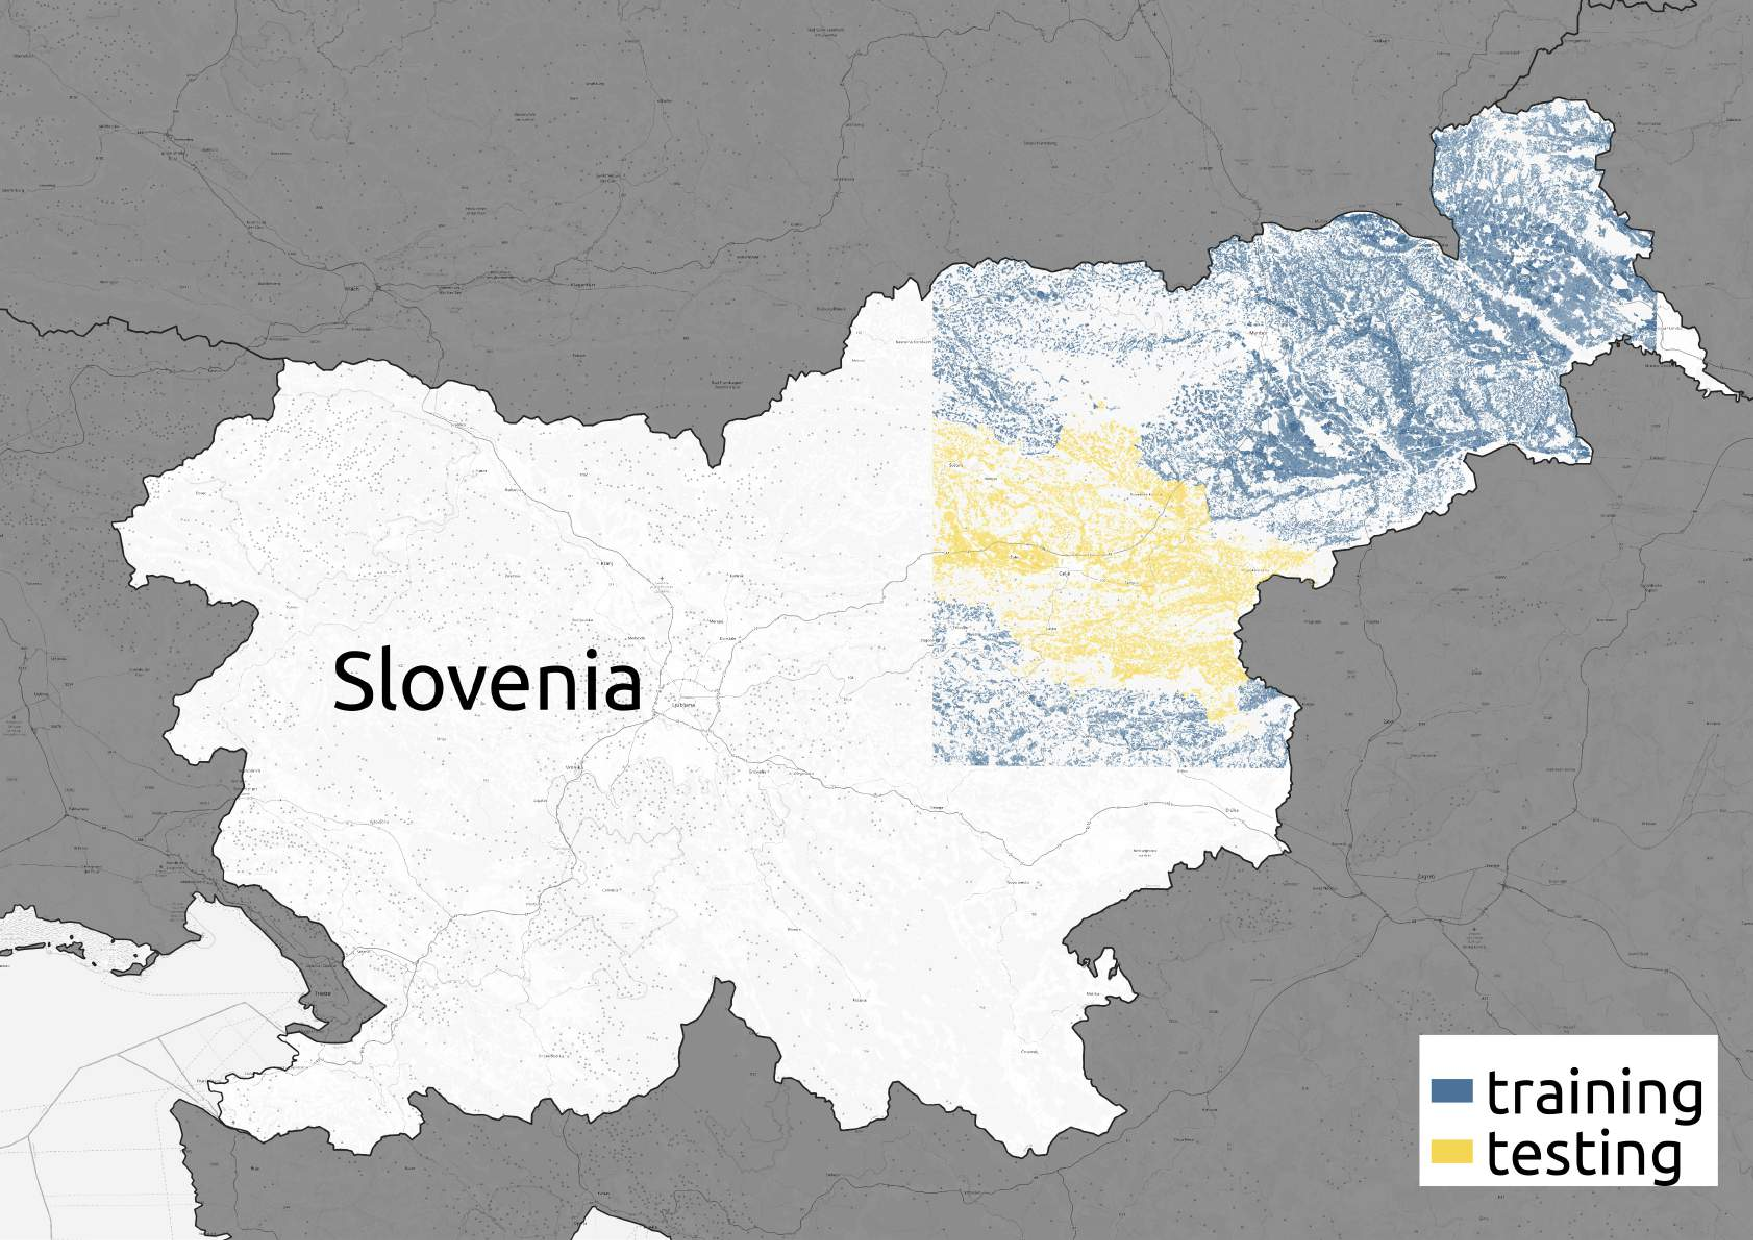
\includegraphics[width=7.5cm]{images/map_slo3}
  \caption{%
    Schematic illustration of the additional SI-\tilename{T33TWM} dataset located in Slovenia with reference crop parcels mainly covering the north-eastern part of the country.
    While the blue areas are used to evaluate the train and test procedure proposed by \citeauthor{Garnot20:SIT}, the yellow area was set aside in advance.
    This way, we ensured to have an extra regionally differentiated test set that does not suffer from the issue of spatial autocorrelation.
  }
  \label{fig:map_slo}
\end{figure}
}

\newcommand{\figDatasetStatistics}{%
\newsavebox{\imagebox}%
\begin{figure}[t]
  \centering
  \savebox{\imagebox}{\pgfplotstablesort[
  col sep=comma, 
  sort cmp=float >,
  sort key={Absolute Occurrence}, 
]
{\datatablesorted}%
{./data/S_top20S.txt}%
% {/home/koerner/doc/papers/2020_RC/Reproducibility_Challenge_2020/data/S_top20S.txt}%
%
\begin{tikzpicture}%[trim axis left,trim axis right]
  \begin{axis}[
    width=.35\linewidth,
    height=4cm,
    crop bar,
    ymode = log, log origin=infty, log ticks with fixed point, 
    ymax=1, ymin=.5e-3,
    xtick=data,
    xticklabels from table={\datatablesorted}{Crop Name},
    yticklabels=\empty,
    xlabel=\empty, xlabel style={overlay},
    ylabel=\empty, ylabel style={overlay},
]
    \addplot[freq bar, fill=bluechill] table [x expr=\coordindex, y={Relative Occurrence}]{\datatablesorted};
    \addlegendentry{Slovenia}
  \end{axis}
% \draw (current bounding box.north east) rectangle (current bounding box.south west); % just for debugging
\end{tikzpicture}%}%
  \begin{subfigure}[t]{.32\linewidth}
    \centering
    \raisebox{\dimexpr\ht\imagebox-\height}{%
      \pgfplotstablesort[
  col sep=comma, 
  sort cmp=float >,
  sort key={Absolute Occurrence}, 
]
{\datatablesorted}
{./data/F_top20F.txt}%
% {/home/koerner/doc/papers/2020_RC/Reproducibility_Challenge_2020/data/F_top20F.txt}%
%
\begin{tikzpicture}
  \begin{axis}[
    width=.5\linewidth,
    width=.35\linewidth,
    height=4cm,
    crop bar,
    ymode = log, log origin=infty, log ticks with fixed point, 
    ymax=1, ymin=.5e-3,
    xtick=data,
    xticklabels from table={\datatablesorted}{Crop Name},
    ylabel style={inner sep=0pt},
]
    \addplot[freq bar, fill=fireorange] table [x expr=\coordindex, y={Relative Occurrence}]{\datatablesorted};
    \addlegendentry{France}
  \end{axis}
%  \draw (current bounding box.north west) rectangle (current bounding box.south east);
\end{tikzpicture}%%
    }%
    \caption{%
      The relative class occurrences of the crop types in the FR-\tilename{T31TFM} dataset provided by the authors of the reproduced paper.
    }
    \label{fig:fr_top_20_bar}
  \end{subfigure}%
  \hfill%
  \begin{subfigure}[t]{.32\linewidth}
    \centering\raisebox{\dimexpr\ht\imagebox-\height}{%
      \pgfplotstablesort[
  col sep=comma, 
  sort cmp=float >,
  sort key={Absolute Occurrence}, 
]
{\datatablesorted}%
{./data/S_top20S.txt}%
% {/home/koerner/doc/papers/2020_RC/Reproducibility_Challenge_2020/data/S_top20S.txt}%
%
\begin{tikzpicture}%[trim axis left,trim axis right]
  \begin{axis}[
    width=.35\linewidth,
    height=4cm,
    crop bar,
    ymode = log, log origin=infty, log ticks with fixed point, 
    ymax=1, ymin=.5e-3,
    xtick=data,
    xticklabels from table={\datatablesorted}{Crop Name},
    yticklabels=\empty,
    xlabel=\empty, xlabel style={overlay},
    ylabel=\empty, ylabel style={overlay},
]
    \addplot[freq bar, fill=bluechill] table [x expr=\coordindex, y={Relative Occurrence}]{\datatablesorted};
    \addlegendentry{Slovenia}
  \end{axis}
% \draw (current bounding box.north east) rectangle (current bounding box.south west); % just for debugging
\end{tikzpicture}%%
    }%
    \caption{%
      The class distribution of the 20 most frequent classes of the newly constructed SI-\tilename{T33TWM} dataset.
    }
    \label{fig:sl_top_20_bar}
  \end{subfigure}%
  \hfill%
  \begin{subfigure}[t]{.32\linewidth}
    \centering\raisebox{\dimexpr\ht\imagebox-\height}{%
      \pgfplotstablesort[
  col sep=comma, 
  sort cmp=float >,
  sort key={France Absolute Occurrence}, 
]
{\datatablesorted}%
{./data/FS_top20F.txt}%
% {/home/koerner/doc/papers/2020_RC/Reproducibility_Challenge_2020/data/FS_top20F.txt} %
%
\begin{tikzpicture}
\begin{axis}[
    width=.5\linewidth,
    width=.35\linewidth,
    height=4cm,
    crop bar,
    bar width=.75mm,
    bar width=.9mm,
    ymode = log, log origin=infty, log ticks with fixed point, 
    ymax=1, ymin=.5e-3,
    xtick=data,
    xticklabels from table={\datatablesorted}{Crop Name},
    yticklabels=\empty,
    xlabel=\empty, xlabel style={overlay},
    ylabel=\empty, ylabel style={overlay},
]
    \addplot[freq bar, fill=fireorange] table [x expr=\coordindex, y={France Relative Occurrence}]{\datatablesorted};
%    \addlegendentry{France}

    \addplot[freq bar, fill=bluechill] table [x expr=\coordindex, y={Slovenia Relative Occurrence}]{\datatablesorted};
%    \addlegendentry{Slovenia}
\end{axis}
% \draw (current bounding box.north east) rectangle (current bounding box.south west); % just for debugging
\end{tikzpicture}%%
    }%
    \caption{%
%      A comparison of the in \subref{fig:fr_top_20_bar} shown class distribution and the relative occurrence of these classes in the new SI-\tilename{T33TWM} dataset. 
      A comparison of the class distribution and the relative occurrences of these classes \subref{fig:fr_top_20_bar} in the new SI-\tilename{T33TWM} dataset. 
      This shows that training and testing on the SI-\tilename{T33TWM} while using the top-20-F labels will lead to fewer classes in total.
    }
    \label{fig:top20F_for_S}
  \end{subfigure}

  \caption{%
    Statistics on the different datasets used in this study. 
    As the data harmonisation was done by hand, the class names of one dataset might include differently named crop types from the other dataset and vice versa. 
    We point out that the relative occurrence is indicated in $\log$-scale, highlighting the strong class imbalance towards meadow.
  }
  \label{fig:dataset_stats}
\end{figure}
}
../openreview/tables.tex

